\documentclass[11pt]{article}
\usepackage[a4paper, margin=2.54cm]{geometry}
\usepackage[utf8]{inputenc}
\usepackage[spanish]{babel}
\usepackage[spanish]{layout}
\usepackage[article]{ragged2e}
\usepackage{textcomp}
\usepackage{subcaption}
\usepackage{graphicx}
\usepackage{booktabs}
\usepackage{siunitx}
\usepackage{pgfplotstable}

\pgfplotsset{compat=1.16}

\sisetup{
  round-mode          = places,
  round-precision     = 4,
}

\begin{document}

\title{
  TRABAJO PRÁCTICO N° 1\\
  \large Estado de la arboleda en el sur de Buenos Aires
}
\author{
  Farizano, Juan Ignacio\\
  \and
  Mellino, Natalia
}
\date{}
\maketitle
\newpage

\tableofcontents
\newpage

\section{Introducción}
\textbf{Motivación del problema:}

\begin{justify}
  En el año 2011 se realizó un Censo Forestal Urbano Público en dos
  comunas del sur de Buenos Aires, en este informe analizaremos los datos de
  dicho censo con el objetivo de determinar el estado actual del arbolado urbano 
  público.\\
  Las variables incluidas en la base de datos dada se describen a continuación.
\end{justify}
% Tabla de variables
\begin{center}
  \begin{tabular}{| c | p{9cm} | c |}
    \hline
    \textbf{Nombre} & \textbf{Descripción} & \textbf{Tipo de variable} \\ \hline
    ID & Identificación del árbol. & Cualitativa nominal \\ \hline
    Altura & Altura de cada árbol, medida en metros (m). Observación: si un árbol
    mide 12,7 m se tomará como dato “12”, truncando los valores a la unidad. & 
    Cuantitativa continua \\ \hline
    Diámetro & Diámetro de cada árbol, medido en centímetros (cm). & 
    Cuantitativa continua \\ \hline
    Inclinación & Ángulo que forma el tronco del árbol respecto a una perpendicular al suelo,
    medido en grados (°). Indica el grado de inclinación del árbol. &
    Cuantitativa continua \\ \hline
    Especie & Especie a la que pertenece el árbol, dentro de las siguientes
    categorías: Eucalipto, Jacarandá, Palo Borracho, Casuarina, Fresno, Ceibo,
    Ficus, Álamo, Acacia. & Cualitativa nominal \\ \hline
    Origen & Procedencia de la especie: Exótico, Nativo/Autóctono, 
    No Determinado. & Cualitativa nominal \\ \hline
    Brotes & Número de brotes jóvenes crecidos durante el último año. &
    Cuantitativa discreta \\ \hline
  \end{tabular}
\end{center}

\newpage

\section{Análisis univariado}

\subsection{Altura}

\begin{table}[h!]
  \begin{center}   
	  \pgfplotstabletypeset[
      multicolumn names,
      col sep=semicolon,
      string type,
      display columns/0/.style={
		    column name=\textbf{Valores},
		    column type={c}},
      display columns/1/.style={
		    column name=\textbf{frecAbs},
        column type={r}},
      display columns/2/.style={
		    column name=\textbf{frecAbsAcum},
		    column type={r}},
      display columns/3/.style={
		    column name=\textbf{frecRel},
        column type={S}},
      display columns/4/.style={
        column name=\textbf{frecRelAcum},
      column type={S}},
      every head row/.style={before row=\toprule,after row=\midrule},
      every last row/.style={after row=\bottomrule},
      every first column/.style={column type/.add={|}{}},
      every last column/.style={column type/.add={}{|}},
    ]{tablaAltura.csv}
    \caption{Tabla de frecuencia.}
    \label{tab:tablaAltura}
  \end{center}
\end{table}

\begin{figure}[h!]
  \begin{center}
    \begin{subfigure}[b]{0.49\linewidth}
      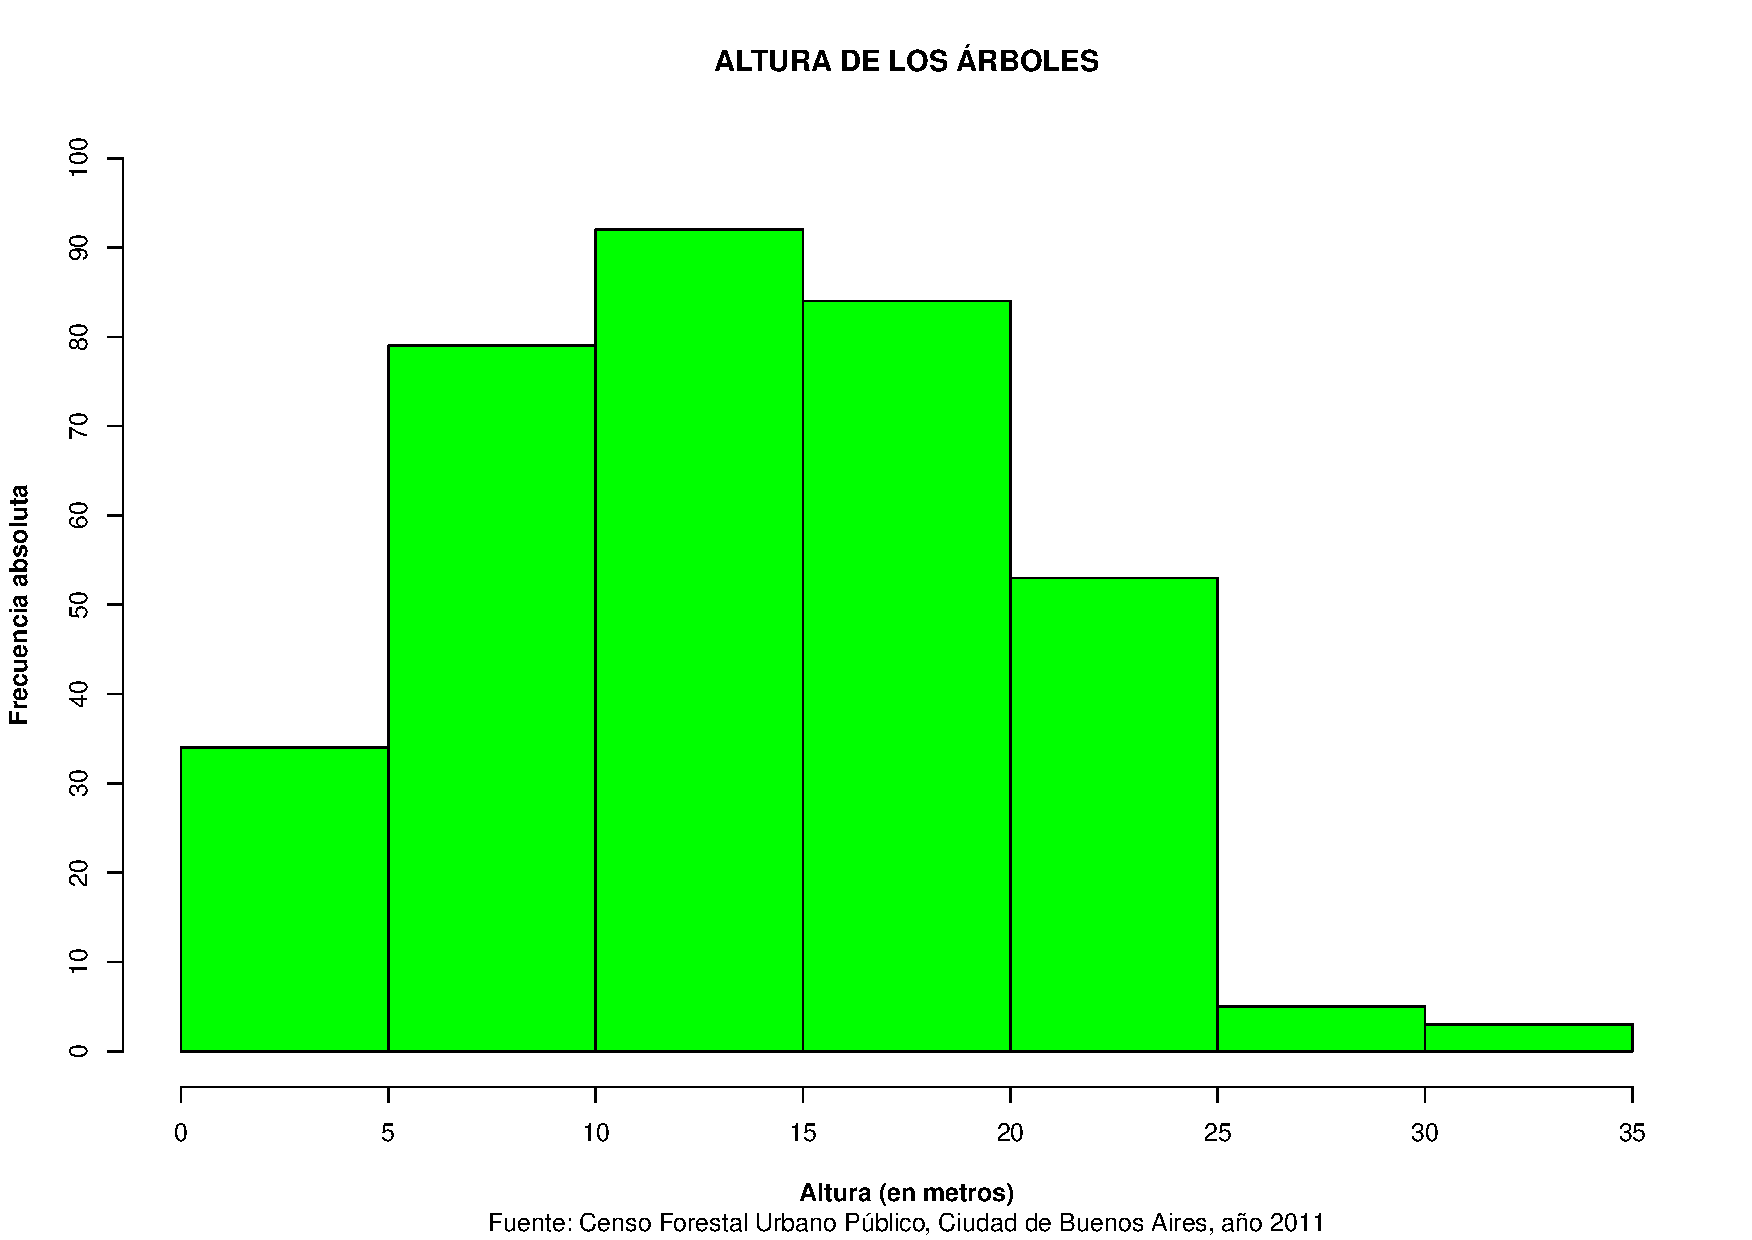
\includegraphics[width=\linewidth]{histAltura.pdf}
      \caption{Histograma.}
      \label{fig:histAltura}
    \end{subfigure}
    \begin{subfigure}[b]{0.49\linewidth}
      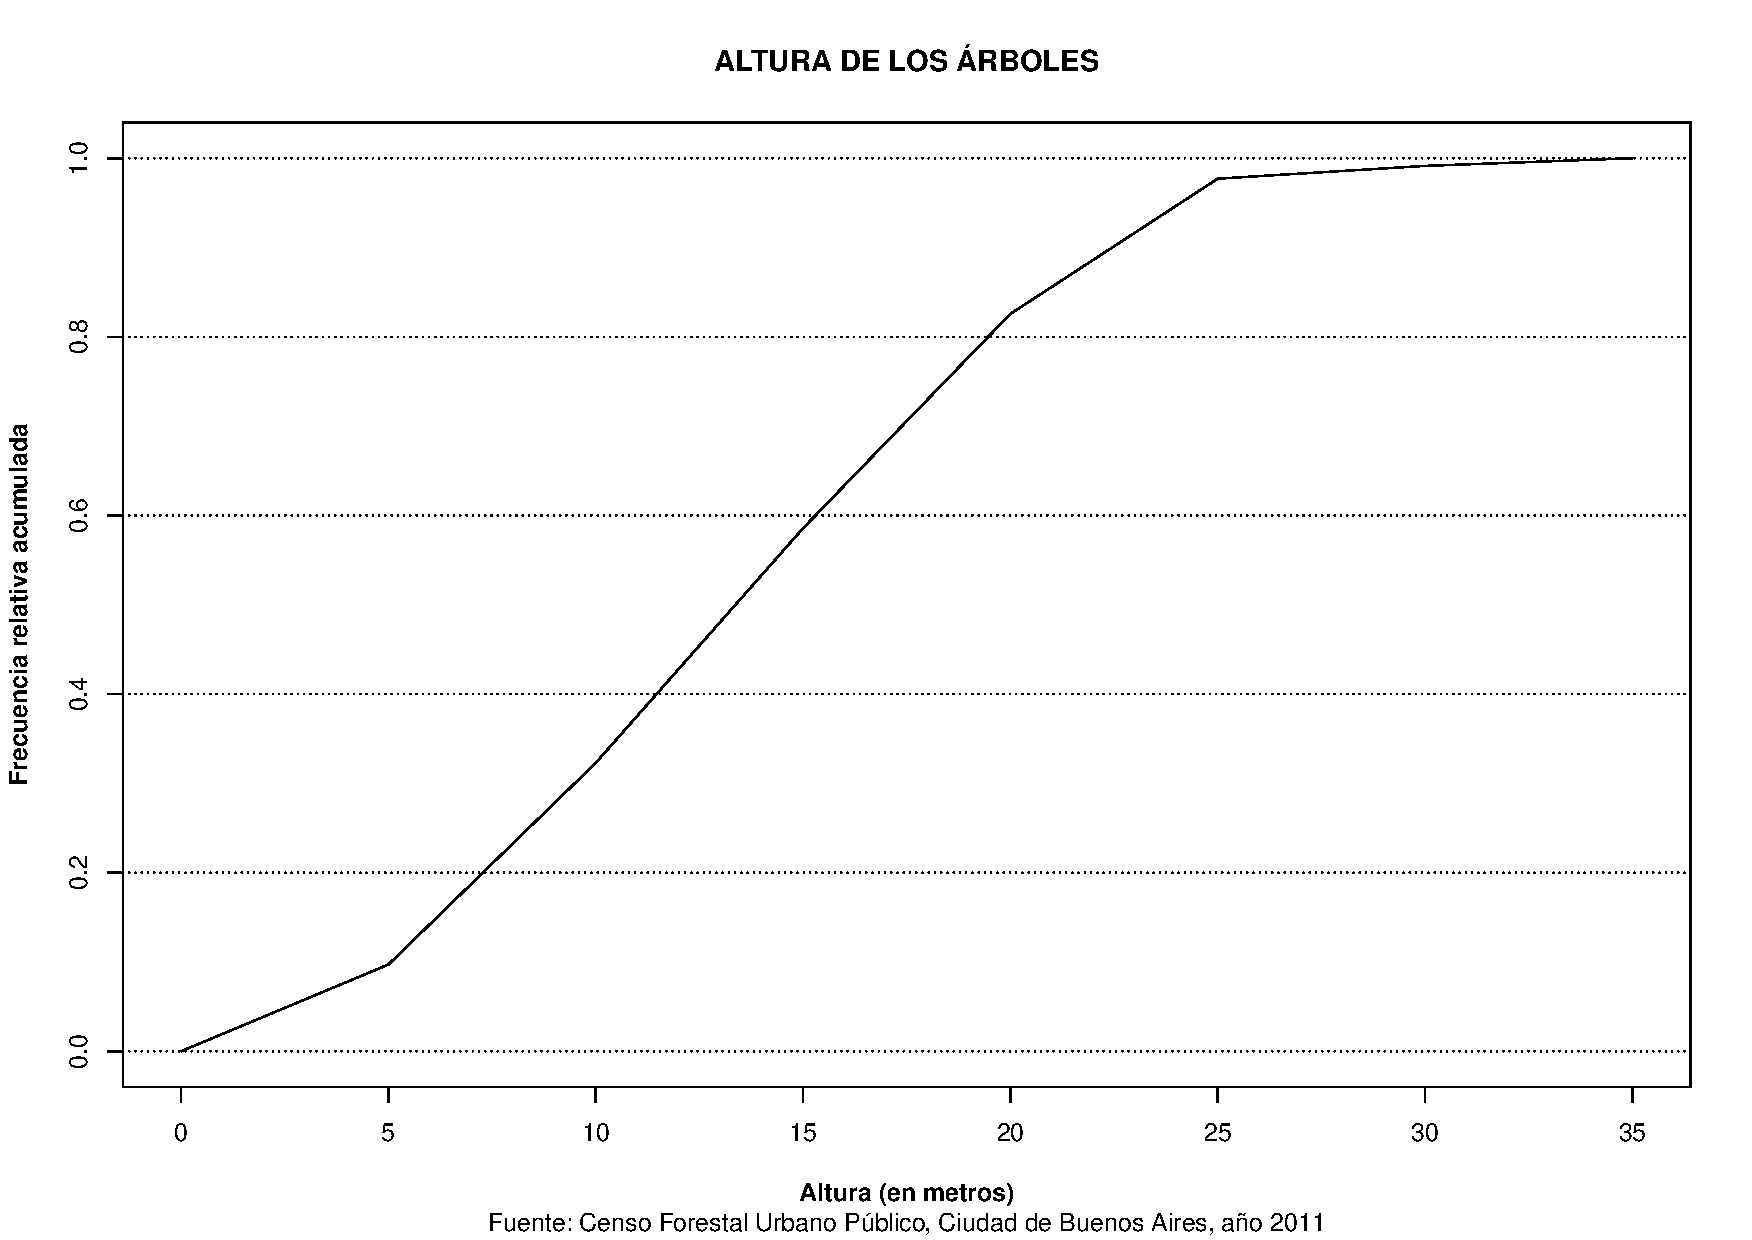
\includegraphics[width=\linewidth]{acumAltura.pdf}
      \caption{Polígono acumulativo.}
      \label{fig:acumAltura}
    \end{subfigure}
  \end{center}  
\end{figure}

\begin{justify}
  El gráfico \ref{fig:histAltura} es unimodal y asimétrico hacia la derecha,
  donde se puede observar
  que una mayor cantidad de árboles tienen una altura entre 10 y 15 mts.
  Si se observa el polígono acumulativo de la figura \ref{fig:acumAltura} 
  junto con la tabla 1 se puede ver que aproximadamente el 97\% de la arboleda 
  presenta una altura inferior a 25 mts. La altura promedio es de 14.02mts.
\end{justify}

\subsection{Diámetro}
\subsection{Inclinación}
\subsection{Especie}
\subsection{Origen}
\subsection{Brotes}

\section{Análisis bivariado}
\subsection{Origen/Especie}
\subsection{Brotes/Especie}

\end{document}
